% Mestre em LaTeX - v0.2
% Copyleft 2008-2010 Bruno C. Vellutini - http://organelas.com/
%
% Permission is hereby granted, free of charge, to any person obtaining a copy
% of this software and associated documentation files (the "Software"), to deal
% in the Software without restriction, including without limitation the rights
% to use, copy, modify, merge, publish, distribute, sublicense, and/or sell
% copies of the Software, and to permit persons to whom the Software is
% furnished to do so, subject to the following conditions:
%
% THE SOFTWARE IS PROVIDED "AS IS", WITHOUT WARRANTY OF ANY KIND, EXPRESS OR
% IMPLIED, INCLUDING BUT NOT LIMITED TO THE WARRANTIES OF MERCHANTABILITY,
% FITNESS FOR A PARTICULAR PURPOSE AND NONINFRINGEMENT. IN NO EVENT SHALL THE
% AUTHORS OR COPYRIGHT HOLDERS BE LIABLE FOR ANY CLAIM, DAMAGES OR OTHER
% LIABILITY, WHETHER IN AN ACTION OF CONTRACT, TORT OR OTHERWISE, ARISING FROM,
% OUT OF OR IN CONNECTION WITH THE SOFTWARE OR THE USE OR OTHER DEALINGS IN
% THE SOFTWARE.
%
% Ou seja, utilize e modifique os arquivos como desejar.
% 
% Para mais informações visite http://code.google.com/p/mestre-em-latex/

% Classe do documento
\documentclass[twoside,a4paper,11pt]{report}

% Pacotes e comandos customizados
%%% Pacotes utilizados %%%

%% Codificação e formatação básica do LaTeX
% Suporte para português (hifenação e caracteres especiais)
\usepackage[english,brazilian]{babel}

% Codificação do arquivo
\usepackage[utf8]{inputenc}

% Mapear caracteres especiais no PDF
\usepackage{cmap}

% Codificação da fonte
\usepackage[T1]{fontenc}

% Essencial para colocar funções e outros símbolos matemáticos
\usepackage{amsmath,amssymb,amsfonts,textcomp}

%% Layout
% Customização do layout da página, margens espelhadas
\usepackage[twoside]{geometry}
% Aumenta as margens internas para espiral
\geometry{bindingoffset=10pt}
% Só pra ajustar o layout
\setlength{\marginparwidth}{90pt}
%\usepackage{layout}

% Para definir espaçamento entre as linhas
\usepackage{setspace}

% Espaçamento do texto para o frame
\setlength{\fboxsep}{1em}

% Faz com que as margens tenham o mesmo tamanho horizontalmente
%\geometry{hcentering}

%% Elementos Gráficos
% Para incluir figuras (pacote extendido)
\usepackage[]{graphicx}

% Suporte a cores
\usepackage{color}

% Criar figura dividida em subfiguras
\usepackage{subfig}
\captionsetup[subfigure]{style=default, margin=0pt, parskip=0pt, hangindent=0pt, indention=0pt, singlelinecheck=true, labelformat=parens, labelsep=space}

% Caso queira guardar as figuras em uma pasta separada
% (descomente e) defina o caminho para o diretório:
%\graphicspath{{./figuras/}}

% Customizar as legendas de figuras e tabelas
\usepackage{caption}

% Criar ambientes com 2 ou mais colunas
\usepackage{multicol}

% Ative o comando abaixo se quiser colocar figuras de fundo (e.g., capa)
%\usepackage{wallpaper}
% Exemplo para inserir a figura na capa está no arquivo pre.tex (linha 7)
% Ajuste da posição da figura no eixo Y
%\addtolength{\wpYoffset}{-140pt}
% Ajuste da posição da figura no eixo X
%\addtolength{\wpXoffset}{36pt}

%% Tabelas
% Elementos extras para formatação de tabelas
\usepackage{array}

% Tabelas com qualidade de publicação
\usepackage{booktabs}

% Para criar tabelas maiores que uma página
\usepackage{longtable}

% adicionar tabelas e figuras como landscape
\usepackage{lscape}

%% Lista de Abreviações
% Cria lista de abreviações
\usepackage[notintoc,portuguese]{nomencl}
\makenomenclature

%% Notas de rodapé
% Lidar com notas de rodapé em diversas situações
\usepackage{footnote}

% Notas criadas nas tabelas ficam no fim das tabelas
\makesavenoteenv{tabular}

%% Links dinâmicos
% Suporte para hipertexto, links para referências e figuras
\usepackage{hyperref}
% Configurações dos links e metatags do PDF a ser gerado
\hypersetup{colorlinks=true, linkcolor=blue, citecolor=blue, filecolor=blue, pagecolor=blue, urlcolor=green,
            pdfauthor={Nome do Autor},
            pdftitle={Título do Projeto},
            pdfsubject={Assunto do Projeto},
            pdfkeywords={palavra-chave, palavra-chave, palavra-chave},
            pdfproducer={Latex},
            pdfcreator={pdflatex}}

% Conta o número de páginas
\usepackage{lastpage}

%% Referências bibliográficas e afins
% Formatar as citações no texto e a lista de referências
\usepackage{natbib}

% Adicionar bibliografia, índice e conteúdo na Tabela de conteúdo
% Não inclui lista de tabelas e figuras no índice
\usepackage[nottoc,notlof,notlot]{tocbibind}

%% Pontuação e unidades
% Posicionar inteligentemente a vírgula como separador decimal
\usepackage{icomma}

% Formatar as unidades com as distâncias corretas
\usepackage[tight]{units}

%% Cabeçalho e rodapé
% Controlar os cabeçalhos e rodapés
\usepackage{fancyhdr}
% Usar os estilos do pacote fancyhdr
\pagestyle{fancy}
\fancypagestyle{plain}{\fancyhf{}}
% Limpar os campos do cabeçalho atual
\fancyhead{}
% Número da página do lado esquerdo [L] nas páginas ímpares [O] e do lado direito [R] nas páginas pares [E]
\fancyhead[LO,RE]{\thepage}
% Nome da seção do lado direito em páginas ímpares
\fancyhead[RO]{\nouppercase{\rightmark}}
% Nome do capítulo do lado esquerdo em páginas pares
\fancyhead[LE]{\nouppercase{\leftmark}}
% Limpar os campos do rodapé
\fancyfoot{}
% Omitir linha de separação entre cabeçalho e conteúdo
\renewcommand{\headrulewidth}{0pt}
% Omitir linha de separação entre rodapé e conteúdo
\renewcommand{\footrulewidth}{0pt}
% Altura do cabeçalho
\headheight 13.6pt

%% Inserir comentários no texto
% Marcar mudanças e fazer comentários
%\usepackage[margins]{trackchanges}
% Iniciais do autor
%\renewcommand{\initialsTwo}{bcv}
% Notas na margem interna
%\reversemarginpar

%% Comandos customizados

% Espécie e abreviação
\newcommand{\subde}{\emph{Clypeaster subdepressus}}
\newcommand{\subsus}{\emph{C.~subdepressus}}

% Título do projeto
\newcommand{\titulo}{Título original do projeto}
\newcommand{\nomedoaluno}{Nome Completo do Aluno}

%% Pacotes não implementados
% Para não sobrar espaços em branco estranhos
%\widowpenalty=1000
%\clubpenalty=1000


% Início do texto
\begin{document}

% Capa
\begin{titlepage}
% Se quiser uma figura de fundo na capa ative o pacote wallpaper
% e descomente a linha abaixo.
% \ThisCenterWallPaper{0.8}{nomedafigura}

\begin{center}
{\LARGE \nomedoaluno}
\par
\vspace{200pt}
{\Huge \titulo}
\par
\vfill
\textbf{{\large São Paulo}\\
{\large 2009}}
\end{center}
\end{titlepage}

% A partir daqui páginas sem cabeçalho
\pagestyle{empty}
% Faz com que a página seguinte sempre seja ímpar (insere pg em branco)
\cleardoublepage

% Números das páginas em algarismos romanos
\pagenumbering{roman}

% Página de Rosto
\begin{center}
{\LARGE \nomedoaluno}
\par
\vspace{200pt}
{\Huge \titulo}
\end{center}
\par
\vspace{90pt}
\hspace*{175pt}\parbox{7.6cm}{{\large Dissertação apresentada ao Instituto de Biociências da Universidade de São Paulo, para a obtenção de Título de Mestre em Ciências, na Área de XXXXXXXX.}}

\par
\vspace{1em}
\hspace*{175pt}\parbox{7.6cm}{{\large Orientador: Nome do Orientador}}

\par
\vfill
\begin{center}
\textbf{{\large São Paulo}\\
{\large 2009}}
\end{center}

\newpage

% Ficha Catalográfica
\hspace{8em}\fbox{\begin{minipage}{10cm}
Aluno, Nome C.

\hspace{2em}\titulo

\hspace{2em}\pageref{LastPage} páginas

\hspace{2em}Dissertação (Mestrado) - Instituto de Biociências da Universidade de São Paulo. Departamento de XXXXXXXX.

\begin{enumerate}
\item Palavra-chave
\item Palavra-chave
\item Palavra-chave
\end{enumerate}
I. Universidade de São Paulo. Instituto de Biociências. Departamento de XXXXXXXX.

\end{minipage}}
\par
\vspace{2em}
\begin{center}
{\LARGE\textbf{Comissão Julgadora:}}

\par
\vspace{10em}
\begin{tabular*}{\textwidth}{@{\extracolsep{\fill}}l l}
\rule{16em}{1px} 	& \rule{16em}{1px} \\
Prof. Dr. 		& Prof. Dr. \\
Nome			& Nome
\end{tabular*}

\par
\vspace{10em}

\parbox{16em}{\rule{16em}{1px} \\
Prof. Dr. \\
Nome do Orientador}
\end{center}

\newpage

% Dedicatória
% Posição do texto na página
\vspace*{0.75\textheight}
\begin{flushright}
  \emph{Dedicatória...}
\end{flushright}

\newpage

% Epígrafe
\vspace*{0.4\textheight}
\noindent{\LARGE\textbf{Exemplo de epígrafe}}
% Tudo que você escreve no verbatim é renderizado literalmente (comandos não são interpretados e os espaços são respeitados)
\begin{verbatim}
O que é bonito?
É o que persegue o infinito;
Mas eu não sou
Eu não sou, não…
Eu gosto é do inacabado,
O imperfeito, o estragado, o que dançou
O que dançou…
Eu quero mais erosão
Menos granito.
Namorar o zero e o não,
Escrever tudo o que desprezo
E desprezar tudo o que acredito.
Eu não quero a gravação, não,
Eu quero o grito.
Que a gente vai, a gente vai
E fica a obra,
Mas eu persigo o que falta
Não o que sobra.
Eu quero tudo que dá e passa.
Quero tudo que se despe,
Se despede, e despedaça.
O que é bonito…
\end{verbatim}
\begin{flushright}
Lenine e Bráulio Tavares
\end{flushright}

\newpage

% Agradecimentos

% Espaçamento duplo
\doublespacing

\noindent{\LARGE\textbf{Agradecimentos}}

Agradeço ao meu orientador, ao meu co-orientador, aos meus colaboradores, aos técnicos, à seção administrativa, à fundação que liberou verba para minhas pesquisas, aos meus amigos, à minha família e ao meu grande amor.

\newpage

\vspace*{10pt}
% Abstract
\begin{center}
  \emph{\begin{large}Resumo\end{large}}\label{resumo}
\vspace{2pt}
\end{center}
% Pode parecer estranho, mas colocar uma frase por linha ajuda a organizar e reescrever o texto quando necessário.
% Além disso, ajuda se você estiver comparando versões diferentes do mesmo texto.
% Para separar parágrafos utilize uma linha em branco.
\noindent
Esta, quem sabe, é a parte mais importante do seu trabalho.
É o que a maioria das pessoas vai ler (além do título).
Seja objetivo sem perder conteúdo.
Um bom resumo explica porquê este trabalho é interessante, relata como foi feito, o que foi encontrado, contextualiza os resultados e delineia conclusões.
\par
\vspace{1em}
\noindent\textbf{Palavras-chave:} palavra1, palavra2, palavra3
\newpage

% Criei a página do abstract na mão, por isso tem bem mais comandos do que o resumo acima, apesar de serem idênticas.
\vspace*{10pt}
% Abstract
\begin{center}
  \emph{\begin{large}Abstract\end{large}}\label{abstract}
\vspace{2pt}
\end{center}

% Selecionar a linguagem acerta os padrões de hifenação diferentes entre inglês e português.
\selectlanguage{english}
\noindent
This is the most important part of your work.
This is what most people will read.
Be concise without omitting content.
A good abstract explains why this is an interesting study, tells how it was done, what was found, contextualizes the results and set conclusions.
\par
\vspace{1em}
\noindent\textbf{Keywords:} word1, word2, word3

% Voltando ao português...
\selectlanguage{brazilian}

\newpage

% Lista de figuras
\listoffigures

% Lista de tabelas
\listoftables

% Abreviações
% Para imprimir as abreviações siga as instruções em 
% http://code.google.com/p/mestre-em-latex/wiki/ListaDeAbreviaturas
\printnomenclature

% Índice
\tableofcontents
   % Capa, prefácio e afins
% Faz com que o ínicio do capítulo sempre seja uma página ímpar
\cleardoublepage
% Inclui o cabeçalho definido no meta.tex
\pagestyle{fancy}
% Números das páginas em arábicos
\pagenumbering{arabic}

\chapter{Introdução (capítulo 1)}\label{intro}
\section{Incluindo citações}\label{intro:historico}

% O comando \label{nome} define o marcador da parte especificada.
% Você pode citar esta seção usando o comando \ref{nome}.
% O "~" evita uma quebra de linha entre as palavras.
O Capítulo~\ref{intro} é uma introdução ao contexto do projeto.
Vou exemplificar alguns comandos básicos e úteis para uma dissertação como incluir citações \citep{Sand-Jensen2007} ou ``aspas''.
% Como o % representa um comentário e não é compilado, para fazê-lo aparecer no texto você precisa colocar uma "\" antes, como abaixo.
Apenas \unit[4]{\%} do texto está contido em subsubseções.

% Veja mais formas de fazer citações no texto da documentação do natbib.
O \texttt{natbib} é bastante flexível \citep[ver detalhes em][]{Kirk2008}.
\citet{Emlet1987} mostra outro modo de citar trabalhos no texto e como grafar o nome das espécies \emph{Drosophila melagonaster} e \subde\ usando o comando \texttt{$\backslash$emph} e um comando customizado, respectivamente.
% Comandos como o utilizado para incluir o nome da espécie (subde e subsus) devem ser seguidos de uma \ para inserir um espaço antes da próxima palavra.
% Esta \ não precisa ser utilizada quando o comando é seguido de ponto ou vírgula.
\citet{Day2006} não usaram papilas de \subsus.
% O pacote icomma permite usar a vírgula como separador decimal, já que o comportamento padrão do LaTeX é inserir um espaço maior após uma vírgula.
O resultado de \subsus\ é 22,2.

\section{Referenciando seções do texto}\label{intro:contexto}

Mencionei na seção~\ref{intro:historico} como citar um capítulo, agora podemos citar o Capítulo~\ref{cap2}.
	% Capítulo 1: Introdução
\pagestyle{empty}
\cleardoublepage
\pagestyle{fancy}
\chapter{Um assunto legal (capítulo 2)}\label{cap2}

\section{Introdução}\label{cap2:intro}

Se desejar inclua um resumo antes desta introdução usando o modelo do \emph{abstract} que está no arquivo \texttt{pre.tex}.
Optei por não incluir um resumo por capítulo.

\section{Materiais e Métodos}\label{cap2:mem}

\subsection{Unidades, frações e fórmulas}\label{cap2:mem:unit}

Você pode dividir cada seção em subseções para organizar melhor o conteúdo.

% Usando o pacote units
O pacote \texttt{units} fornece comandos para formatar unidades e frações como \nicefrac{animal}{vegetal} (\nicefrac{A}{V}) e \unitfrac[500]{µm}{s}.
Ou mesmo \unit[7,5]{h} após a elevação.

Note como formatar a unidade de temperatura e outro exemplo de fração à temperatura constante de \unit[24]{°C}; a concentração final foi de 100~\nicefrac{células}{mL}.
Ao invés de usar o pacote \texttt{units} (como no começo do parágrafo) você pode usar o comando \texttt{$\backslash$,} para obter o meio espaço entre o número e sua unidade, com 0,6\,g e 7,7\,g.

Um dos pontos fortes do \LaTeX\ é a praticidade e beleza das fórmulas matemáticas\footnote{Não que isso seja uma fórmula matemática de verdade\ldots, mas isto é uma nota de rodapé ;-)}:
\begin{equation}\label{eq:ind}\notag
IG=\frac{\text{peso úmido da gônada}}{\text{peso úmido do exemplar - (peso úmido da gônada)}}
\end{equation}

% A inserção de fórmulas no meio do texto requer o uso de $fórmula$ (cifrões)
a concentração final foi de $8\times10^5$ e $1\times10^6$ \nicefrac{células}{mL}.
A cultura foi mantida num ciclo de $12:12$ horas.
Também é possível inserir fórmulas no meio do texto como $2,7\pm\unit[1,1]{g}$ ($n=119$), com amostras entre \unit[0,6]{g} e \unit[7,7]{g} e $P=0,007$.


Citando programa de processamento de imagens \emph{ImageJ} \citep{Rasband1997} e a linguagem \emph{R} \citep{R2005} para a morfometria ($P<0,050$).
Os testes estão em fonte \texttt{monoespaçada}, os estágios em \textbf{negrito} e os dados na forma $\text{média} \pm \text{desvio padrão}$.
\subsection{Cultivo das subsubseções}\label{cap2:mem:gametas}

\subsubsection{Embrião}

Você também pode criar subsubseções como essa, caso necessário.

\subsection{Descrições}\label{cap2:mem:micro}

Subseção após a subseção com subsubseção.

\subsubsection{Fêmeas}\label{cap3:res:femeas}

Mais uma subsubseção.

% Outro ambiente útil é o description, como exemplificado abaixo.
\begin{description}
  \item[Estágio1 $(n=27)$:] Descrição minuciosa deste estágio.
    Estou incluindo um pouco de texto extra para mostrar como a formatação fica impecável.
    Uma boa formatação não distrai o leitor e proporciona maior clareza e prazer durante a leitura.
  \item[Estágio2 $(n=25)$:] Descrição minuciosa deste estágio.
    Estou incluindo um pouco de texto extra para mostrar como a formatação fica impecável.
    Uma boa formatação não distrai o leitor e proporciona maior clareza e prazer durante a leitura.
\end{description}

As descrições também podem ser colocadas uma dentro da outra.

\begin{description}
  \item[Tipo1:] Descrição minuciosa.
    Estou incluindo um pouco de texto extra para mostrar como a formatação fica impecável.
    A razão $\frac{\text{núcleo}}{\text{citoplasma}}\times100=51,0\pm\unit[11,9]{\%}$.
  \item[Tipo2:] ~
    \begin{description}
      \item[Subtipo2.1:] Descrição minuciosa deste tipo.
	Estou incluindo um pouco de texto extra para mostrar como a formatação fica impecável.
      \item[Subtipo2.2:] Descrição minuciosa deste tipo.
	Estou incluindo um pouco de texto extra para mostrar como a formatação fica impecável.
    \end{description}
  \item[Tipo3:] Descrição minuciosa deste tipo.
	Estou incluindo um pouco de texto extra para mostrar como a formatação fica impecável.
\end{description}

\subsubsection{Tabelas}\label{cap3:res:morf}

Utilize tabelas como a Tabela~\ref{tab:exemplo}.

% Para criar tabelas
\begin{table}[htbp]
    \caption[Tabela com \texttt{booktabs}]{Exemplo de legenda de tabela criada com o pacote \texttt{booktabs}.}
    \label{tab:exemplo}
    \vspace{1em}
    \centering
    \begin{tabular}{l r@{\,} l}
        \toprule
        Eventos     & \multicolumn{2}{c}{Tempo}\\
        \midrule
        Entrada     & 0   & \\
        Elevação    & 40  & s   \\
        Corrida     & 6   & min \\
        Saída       & 15  & min \\
        \bottomrule
    \end{tabular}
\end{table}

Outra tabela de exemplo onde utilizamos o teste \texttt{t} (Tabela~\ref{tab:areap}).
No caso, o modelo de regressão linear é descrito pela equação $y=0,799x+0,699$.

\begin{table}[htbp]
    \caption[Tabelas com valores de $P$]{Um exemplo de tabela comum em trabalhos científicos mostrando valores de $P$ em uma comparação estatística, $\alpha=0,05$.}
    \label{tab:areap}
    \vspace{1em}
    \centering
    \begin{tabular}{l r r r r r}
        \toprule
        ~	        & Estágio1          & Estágio2      & Estágio3	        & Estágio4\\
        \midrule
        Estágio2	& 1,000		    & -		    & -		        & -\\
        Estágio3	& 0,883		    & 1,000	    & -		        & -\\
        Estágio4	& \textbf{<0,001}   &\textbf{<0,001}& \textbf{<0,001}   & -\\
        \bottomrule
    \end{tabular}
\end{table}

\section{Resultados}\label{cap2:res}

\subsection{Figuras simples}\label{cap2:res:figs}

Subseção de novo, mas coloco algumas figuras para mostrar resultados (Figura~\ref{fig:last}).
Também é possível definir o tamanho da figura relativamente (e.g., metade da largura do texto; Figura~\ref{fig:last2}).

% Veja a documentação para mais detalhes de como inserir figuras
% O texto entre [] na legenda será utilizado na lista de figuras (no preâmbulo), sendo ideal para substituir legendas maiores
\begin{figure}[htbp]
    \centering
    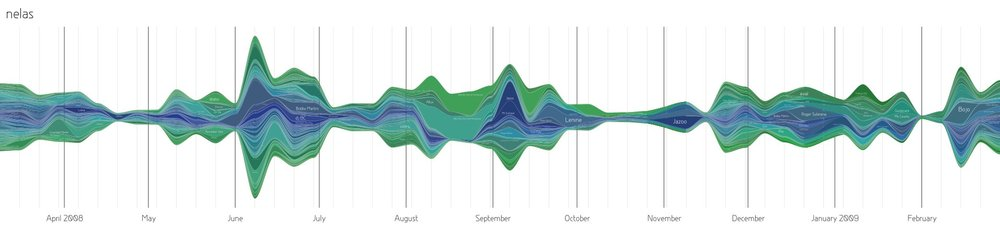
\includegraphics[width=\textwidth]{lastgraph}
    \caption[Figura simples]{Figura abstrata simples com largura igual à largura do texto.}
    \label{fig:last}
\end{figure}

\begin{figure}[htbp]
    \centering
    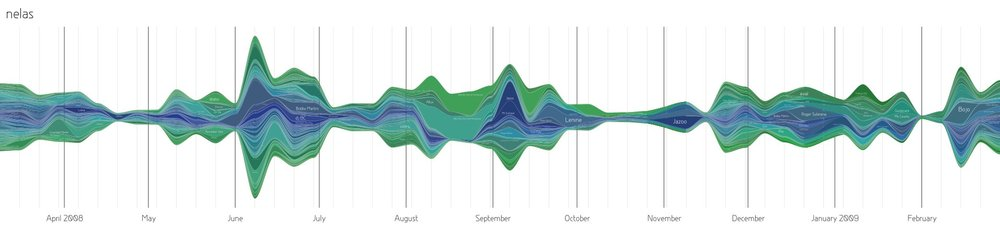
\includegraphics[width=0.5\textwidth]{lastgraph}
    \caption[Outra figura simples]{Figura abstrata simples com largura igual à metade da largura do texto.}
    \label{fig:last2}
\end{figure}

\subsection{Figuras compostas e abreviações}\label{cap2:res:figs2}

Você também pode inserir múltiplas figuras em uma só, permitindo alinhá-las de forma flexível e consistente (ver Figura~\ref{fig:fsm}).

% Usando o pacote nomencl
% Detalhe importante, leia as instruções no site para fazer a lista de abreviações aparecer.
% http://code.google.com/p/mestre-em-latex/wiki/ListaDeAbreviaturas
Para selecionar abreviações que serão incluídas na lista no começo do documento veja o arquivo \texttt{cap2.tex}; como a seguir as células mesenquimais primárias (CMP) iniciam sua ingressão.%
\nomenclature{CMP}{células mesenquimais primárias}

% Note como incluir as sublegendas para cada subfigura (subfloat) e como citá-las na legenda usando o comando subref.
% Note também como incluir as referências às abreviações (nomenclature) utilizadas para que sejam listadas no preâmbulo.
\begin{figure}[htbp]
    \centering
    \subfloat[Subfigura1]{\label{fig:t1}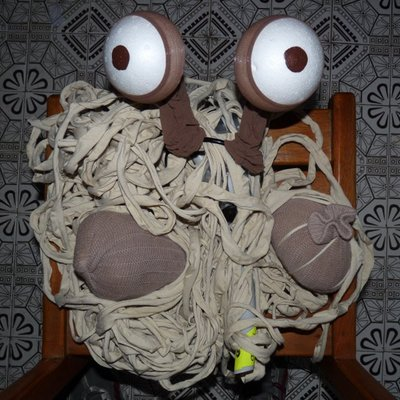
\includegraphics[width=200pt]{fsm}}\vspace{11pt}
    \subfloat[Subfigura2]{\label{fig:t2}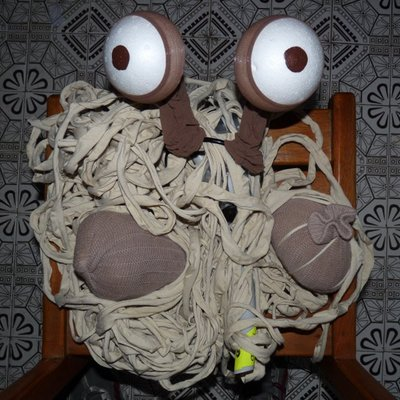
\includegraphics[width=200pt]{fsm}}\\
    \vspace{-18pt}
    \subfloat[Subfigura3]{\label{fig:t3}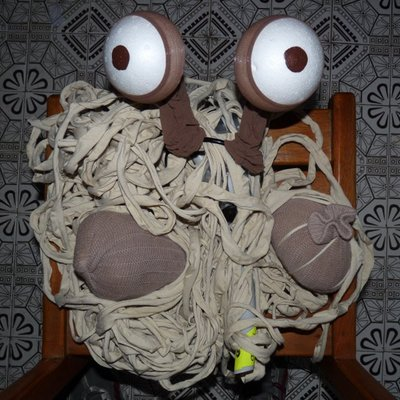
\includegraphics[width=200pt]{fsm}}\vspace{11pt}
    \subfloat[Subfigura4]{\label{fig:t4}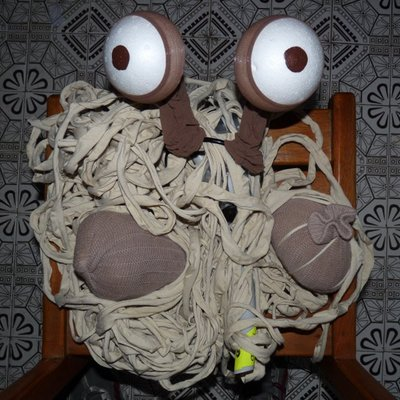
\includegraphics[width=200pt]{fsm}}%
    \caption[Figura com subfiguras]{Exemplo de figura com subfiguras. \subref{fig:t1}~Subfigura1 (\textbf{og}) na lâmina. \subref{fig:t2}~Subfigura2 (\textbf{oppv}). \subref{fig:t3}~Subfigura3 aderida (\textbf{opv}). \subref{fig:t4}~Subfigura4. \textbf{sg}, seio genital; \textbf{ln}, lúmen.}%
    \nomenclature{og}{oogônia}%
    \nomenclature{oppv}{oócitos primários pré-vitelogênicos}%
    \nomenclature{opv}{oócitos primários vitelogênicos}%
    \nomenclature{sg}{seio genital}%
    \nomenclature{ln}{lúmen}
    \label{fig:fsm}
\end{figure}

\section{Discussão}\label{cap2:disc}

A evolução deste caráter pode ser vista de duas formas:

% Este é um dos modos de iniciar uma lista ordenada.
% Note que é possível inserir listas dentro de listas.
\begin{enumerate}
  \item{Condição inicial $\longrightarrow$ Condição final}\label{hipo:1}
    \begin{itemize}
      \item{Primeira conseqüência}
      \item{Segunda conseqüência}
    \end{itemize}
  \item{Outra condição inicial $\longrightarrow$ Condição intermediária $\longrightarrow$ Outra condição final}\label{hipo:2}
    \begin{itemize}
      \item{Conseqüência alternativa}
    \end{itemize}
\end{enumerate}

Você pode citar ítens assinalados, como a hipótese \ref{hipo:1} e a alternativa \ref{hipo:2}.
	% Capítulo 2: ...
\pagestyle{empty}
\cleardoublepage
\pagestyle{fancy}
\chapter{Considerações Finais}

As vezes faz bem sentar e pensar nas considerações finais do seu trabalho, não só para os que lerão o texto, mas para aquele que o escreve.
	% Capítulo 3: Considerações Finais

% Formato da bibliografia
\bibliographystyle{apalike}
% Arquivo .bib
\bibliography{mestre}

% Apêndice(s)
\appendix
\chapter{Primeiro apêndice}
Apêndices são opcionais, mas podem ser usados, por exemplo, para incluir tabelas com os dados brutos.


% Fim do texto
\end{document}
